% 
\newglossaryentry{X}
{
  type=differential-privacy,
  name={$\ensuremath{X} $},
  description={Set of locations for a user. ($R^2$)},
}
\newglossaryentry{Z}
{
  type=differential-privacy,
  name={$\ensuremath{Z} $},
  description={For every $x \in X$ a perturbed location $z \in Z$ is reported.},
}
\newglossaryentry{K}
{
  type=differential-privacy,
  name={$K(x)(Z)$},
  description={Randomization method for $x \in X$ and output $z \in Z$.},
}
\newglossaryentry{Epsilon}
{
  type=differential-privacy,
  name={$\ensuremath{\epsilon} $},
  description={The privacy budget $\epsilon$ determines the amount of noise that is added.
    },
}
\newglossaryentry{Pr}{
  type=differential-privacy,
  name={$Pr(K(x_i) \in (Z))$},
  description={Probability of reporting $x \in X$ for $z \in Z$}
}


\section{Differential privacy} \label{section:dp}
In practice, data is often sent to a central storage point.
This requires trust, and because all data is collected in one place, the risk of private data leakage becomes very high.
By applying \gls{dp}, noise can be added to the data to protect it.
This principle is illustrated in figure \ref{fig:central-dp} with the following actors:
\begin{enumerate}
  \item Trusted curator: The system that receives data from users. It is assumed in this setting that the system is trustworthy and that the data is securely stored.
  \item Adversary: An adversary is someone who uses the data. This could be, for example, a data scientist who wants accurate results or an attacker who wants to obtain as much data as possible.
  \item The users are clients (for example, websites or mobile apps) who entrust their data to a central server.
\end{enumerate}
To a certain extent, a user's privacy would be ensured with differential privacy. \newline

Although differential privacy solves privacy problems, it remains challenging to calibrate the mechanism.
There is an important trade-off between utility and privacy for the adversary.
For example, a data scientist wants accurate data. At the same time, the noise must be sufficient to prevent an attacker from obtaining too much information.
For this reason, a few sections will be devoted to outlining the mathematical background of differential privacy.
We will examine which factors influence this calibration and whether other methods contribute.
Afterward, we will further explain other types of differential privacy (local and geo-indistinguishable) similarly.
\begin{figure}[h!]
  \includesvg[width=1\textwidth]{TheorethicalFramework/Differential privacy/central-dp}
  \caption{General approach for setting up (central) differential privacy.}
  \label{fig:central-dp}
\end{figure}

On the left side are the users, who send their data to the trusted curator.
The trusted curator collects all the data (e.g., a database) and adds noise to the data.
The adversary (right) can access the private data but should not be able to access the non-private data.
%\glsaddall
%\leading{10pt}
%\printglossary[type=differential-privacy, nonumberlist]
%\begin{figure}[h]
%  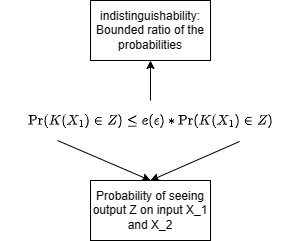
\includegraphics{TheorethicalFramework/Differential privacy/master-thesis-Differential privacy illustration.png}
%  \caption{Randomization function $K$ gives $\epsilon$-differential privacy for all elements in $D_1$ and $D_2$ if they differ at most one element. \citep{dwork_differential_2006}}
%  \label{fig:definition-dp}
%\end{figure}

\newpage
\subsection{Definitions}
We examine the different notations and types of differential privacy we consider in this research.

\subsubsection{$\epsilon$-differential privacy}
Dwork et al. formulated the notion of privacy: Participating in a database should not significantly increase the risk of an individual's privacy being compromised \cite{dwork_differential_2006}.
This is mathematically formulated in the same research named \gls{dp}.
Using the definition of privacy, it is formulated as the maximal possible change when adding or removing a single record \citep{dwork_differential_2006, friedman_data_2010}.
This is reflected using the formal mathematical formulation as formulated by Dwork et al:
\begin{equation}
  {\mathrm{Pr}}[K(D_{1})\in S]\leq\exp(\epsilon)\times{\mathrm{Pr}}[K(D_{2})\in S]
  \label{pure-dp}
\end{equation}
So, given a randomization function $K$, it gives $\epsilon$-differential privacy if dataset $D_1$ and $D_2$ are differing at most one element \citep{dwork_differential_2006}.
The $\epsilon$ determines the amount of noise (privacy budget) \citep{friedman_data_2010}.
The lower the value of $\epsilon$, the higher the privacy guarantee.
In this regard, it is essential for a method that ensures differential privacy to consider this.
For this reason, a common way to calibrate the $\epsilon$ is to calculate the sensitivity.
This value is calculated based on the impact of a function or query on the data.
For example, if there is a method called $sum$ for the summation of data points, the method's sensitivity is 1.
This is because removing one data point would significantly affect the outcome, and $\epsilon$-differential privacy could no longer be guaranteed.
It is also mathematically defined by Dwork et al.:
\begin{equation}
  \Delta f=\operatorname*{max}_{D_{1},D_{2}}\|f(D_{1})-f(D_{2})\|_{1}
  \label{sensitivity-dp}
\end{equation}
\subsubsection{$(\epsilon, \delta)$-differential privacy}
The formal notion of differential privacy has only the privacy budget $\epsilon$ as a parameter.
This formulation is strict, but most methods relax this a little, with $(\epsilon, \delta)$:
\begin{equation}
  {\mathrm{Pr}}[K(D_{1})\in S]\leq\exp(\epsilon)\times{\mathrm{Pr}}[K(D_{2})\in S] + \delta
  \label{approxiate-dp}
\end{equation}
This equation means the sensitivity ($\delta$) loosens the formal definition of differential privacy.
The $\delta$ is added to the upper bound of the exponential, so the desired noise can be higher.
%The purpose of $\epsilon$ now is to calibrate the desired amount of privacy.
To some extent, the delta represents the probability of the algorithm leaking information \citep{aitsam_differential_2021}.
With $\epsilon$-differential privacy, there would be no difference in the case of information leakage ($\delta$ = 0).
However, with $(\epsilon, \delta)$-differential privacy, the information can leak up to the probability of delta.
\newpage
\subsubsection{$\epsilon$-local differential privacy}
As the name suggests, \gls{ldp} is executed on the client side instead of on the server (See Figure \ref{fig:central-dp}).
%The principle of \gls{ldp} is illustrated in figure \ref{fig:local-dp}.
Local differential privacy removes the "trusted" curator (See Figure \ref{fig:local-dp}), preventing sensitive data leakage even if an attacker gains access to the dataset \citep{del_rey_comprehensive_2020}.
The definition for \gls{ldp} is the as for equation \ref{approxiate-dp} with $\delta = 0$ being equal to equation \ref{pure-dp}.
\begin{figure}[ht]
  \includesvg[width=1\textwidth]{TheorethicalFramework/Differential privacy/local-dp}
  \caption{Local differential privacy, which moves the noise-adding step to the client-side.}
  \label{fig:local-dp}
\end{figure}

Local differential privacy has two different frameworks.
It can be set up as interactive or non-interactive \citep{del_rey_comprehensive_2020}.
Where interactive can be distinguished as either sequentially interactive or fully interactive \footnote{Image source: \url{https://www.majos.net/focs_19_talk.pdf}}:
\begin{figure}[H]
  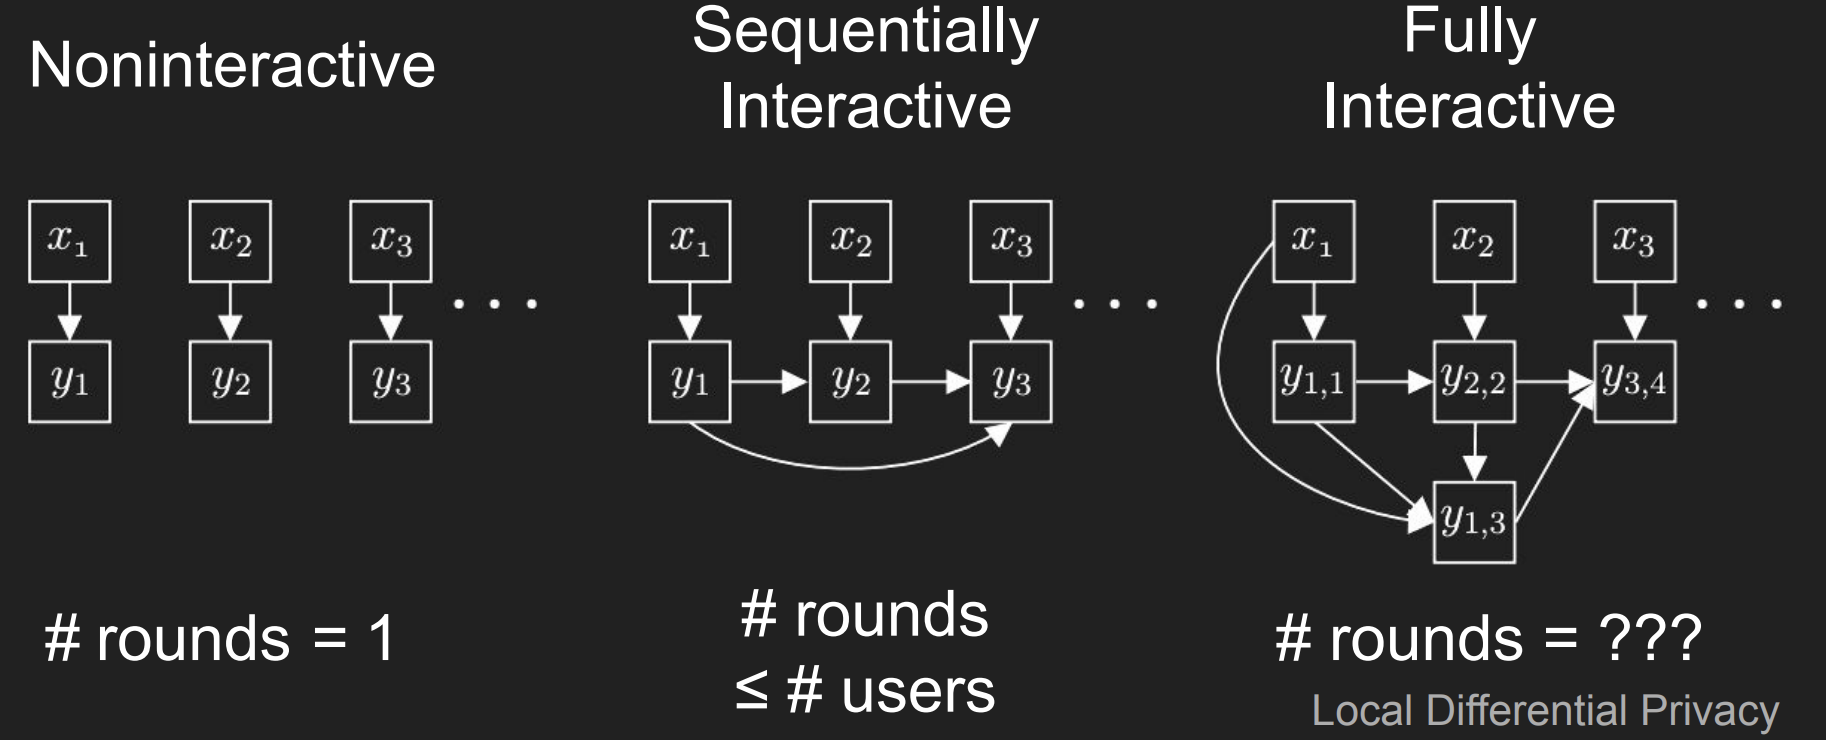
\includegraphics[width=\textwidth]{TheorethicalFramework/nont-interactive-versus-interactive.png}
  \caption{Non-interactive versus sequentially interactive versus fully interactive local differential privacy \citep{joseph_role_2019-1}}
  \label{fig:non-interactive-versus-interactive}
\end{figure}
In the non-interactive framework, the privacy mechanism operates on a single data instance (e.g., users’ smartphones) without requiring interaction with other clients or between data points.
This interaction means that each data point is perturbed independently, and the privacy guarantees are achieved without communication or coordination between the data points.
In the interactive framework, the privacy mechanism involves a process of iterative interactions between users and clients.
Each data point considers other data points' responses to determine its own perturbation or privacy level.
The interactions can occur through a communication channel, where data points exchange information with each other or a trusted mediator.
The iterative nature of the interactive framework allows for refining and improving the privacy guarantees based on the global knowledge of the data set.

In figure \ref{fig:non-interactive-versus-interactive}, the different interactive types are visualized, where the most notable difference is the around of rounds \citep{xiongComprehensiveSurveyLocal2020}.
A sequentially interactive framework passes at most one message between data points.
A fully interactive framework could provide an unknown and unlimited amount of messages between data points.
The interactive framework has unlimited access to other data points, which is most suitable for practical appliances \citep{xiongComprehensiveSurveyLocal2020}.
The practical applications are better because the data points' mutual correlation also contributes to utility \citep{wang_comprehensive_2020}.

\subsubsection{$\epsilon$-geo-indistinguishability} \label{theory:geo-indistinguishability}
The last and most important type of differential privacy for this study is \gls{gi}.
%This is a type of differential privacy that is specifically designed for location data.
\gls{gi} can be applied to preserve privacy using a differential privacy method specific to spatial data \citep{DBLP:journals/corr/abs-1212-1984}.
Consider a local-based system (LBS) that provides a map service to its users (e.g., Google Maps).
The users can query the LBS for a route from their current location to a destination.
%This information is private, and the LBS should not be able to track the user's location.
Instead of the exact (private) location, the LBS should only receive an approximate location enough to provide the service at an adequate level.
This approximation happens entirely locally, so no central server exists.

Users can define a privacy radius $r$ around their location $x$.
A fake location $z$ is generated within this radius based on the Euclidean distance $d$. \newline
The amount of noise within $r$ depends on the privacy budget $\epsilon$.
The privacy budget is based on the privacy level $l$, combined with $r$ to obtain $\epsilon$ using the formula $\epsilon = \frac{l}{r}$. \newline
Calculating the privacy budget is illustrated in the figure below:
\begin{figure}[H]
  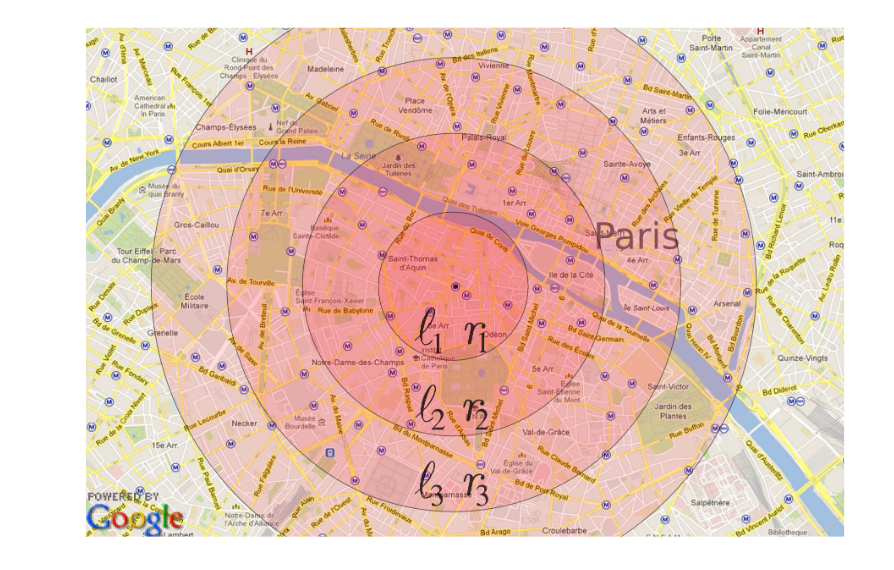
\includegraphics[width=0.5\textwidth]{TheorethicalFramework/geo-indistinguishability.png}
  \caption{Visualisation of radius $r$ with $l$ to provide Geo-indistinguishability mechanism \citep{DBLP:journals/corr/abs-1212-1984}}
  \label{fig:geo-indistinguishability}
\end{figure}

The formula for \gls{gi} to measure if an algorithm preserves $\epsilon$-geo-indistinguishability can be expressed as:
\begin{equation}
  K(x)(y) \le e^{\epsilon * d(x,x')} K(x')(y)
  \label{algo:2d-geo-indistinguishability}
\end{equation}
$K$ is a probability method reporting $x, x' \in X$ as $z \in Z$.
%The intuition of this algorithm looks a lot like that of differential privacy using the La Place method; but includes distance.
The intuition for this definition is that it displays the distinguishability level between two secret locations/points $x$ and $x'$ \citep{chatzikokolakis_constructing_2015}.
An extension of this is called $d_x$-privacy, a more general notation of distance-aware differential privacy.
Therefore, their definition for \gls{gi} is $d_2$-privacy, but is essentially the same as the proof provided for \gls{gi}.
\newpage
\subsection{Mechanisms}
This section explains the various mechanisms used to achieve differential privacy.
The different mechanisms are not limited to the type of \gls{dp}; some can be applied to multiple types.
%The mechanisms are divided into three categories: \gls{dp}, \gls{ldp} and \gls{gi}.
\subsubsection{Randomized response mechanism}
The random response method is relatively simple and was first applied in 1965 by Warner et al.
It was originally used to mask individuals' answers by randomly switching them with predictable randomness \citep{warner_randomized_1965}.
Therefore, the method is mainly used for categorical data.
This method satisfies its own set of requirements for LDP \citep{del_rey_comprehensive_2020}, which differs from the formal definition that was mentioned earlier

Since then, it is still one of the better-known methods, and larger organizations such as Google have used it \citep{erlingsson_rappor_2014}.
They have named their extension RAPPOR and expanded it with bloom filters to be able to collect numerical data as well.
It is possible to ensure $\epsilon$-differential privacy, and it is also possible to preserve \gls{ldp} \citep{del_rey_comprehensive_2020}.
\subsubsection{Laplace mechanism} \label{laplace}
The method that was initially proposed in the differential privacy paper by Dwork et al. is the Laplace algorithm \citep{dwork_differential_2006}.
Therefore, the method configures the $\epsilon$ and $\delta$. A shorthand definition is provided by Rey et al. \citep{del_rey_comprehensive_2020}:
\begin{equation}
  M\left(f\left(x\right),\varepsilon\right)=f\left(x\right)+\left(Z_{1},\ldots,Z_{d}\right)
\end{equation}
The mechanism is based on the Laplace distribution with scale $\lambda f/\epsilon$, where $\lambda f$ is the same as in equation \ref{sensitivity-dp}.
Therefore, the Laplace mechanism is tightly linked to the definition of \gls{dp} \citep{dwork_differential_2006}.
In addition to this, it is also suitable for preserving \gls{ldp} \citep{del_rey_comprehensive_2020}.
One disadvantage is that sensitivity is always required, and this parameter can sometimes be difficult to configure.
Especially when there is no clear function and the entire dataset is perturbed.
This can make finding the right balance between ensuring privacy and utility challenging.

To this end, the sensitivity can be calculated in two forms: global and local.
Global sensitivity is independently calculated over two different datasets and is part of the original definition of \gls{dp} \citep{dwork_differential_2006}.
Usually, this is not the desired situation since local sensitivity always has more context of the dataset in question \citep{nissim_smooth_2007}.
As a result, the trade-off for noise is much more precise, and the balance between utility and privacy is much better.
The definition of local sensitivity is the following \citep{nissim_smooth_2007}.
\begin{equation}
  LS(f,x)=\operatorname*{max}_{x^{\prime}\cdot d(x,x^{\prime})\leq1}|f(x)-f(x^{\prime})|
  \label{local-sensitivity}
\end{equation}
A methodology to calculate the local sensitivity is using the smooth sensitivity method, proposed by the same authors \citep{nissim_smooth_2007}.
This method aims at smoothing out the local sensitivity by focusing on reducing the noise without the risk of revealing more information.
Because it calculates many different configurations, a disadvantage of this method is that it can be computationally expensive.
Also, the introduction of this method makes Laplace preserve $(\epsilon, \delta)$-\gls{dp} instead of pure $\epsilon$-\gls{dp}.

%\subsubsection{Gaussian mechanism} \label{gaussian}
%Another mechanism that works comparably is the Gaussian mechanism.
%This mechanism makes use of the Gaussian distribution to add noise to the data.
%\todo[inline]{Explain more about Gaussian mechanism}
% This means, that if the sensitivity is low, the noise is as well.
% The metric is combined with the privacy budget $\epsilon$ to control the noise that is being added by a mechanism like Laplace \citep{friedman_data_2010}.


%The above attacks mainly target the clustering method after they have been trained. 
%$Various attacks are more focused on data, like 
%\subsection{Evaluation methods} \label{theory:evaluation-dp}
\newpage
